\documentclass{article}
\usepackage{fullpage}
\usepackage{amsmath}
\usepackage{tikz}
\usepackage{bm}
\usepackage{natbib}
\usepackage[hidelinks]{hyperref}
\usepackage{siunitx}
\usepackage{doi}
\usetikzlibrary{decorations.pathreplacing}

\newcommand{\Co}{C}
\newcommand{\vect}{\bm}
\newcommand{\iu}{{i\mkern1mu}}
\newcommand{\TODO}[1]{\textcolor{purple}{TODO: \emph{#1}}}

\title{A high-order correction to the one-dimensional cubicFit transport scheme}
\author{James Shaw}

\begin{document}
\maketitle

A transport scheme is `super-convergent' when its order of convergence is higher on uniform meshes than on non-uniform meshes.
For example, the transport scheme by \citet{skamarock-gassmann2011} is super-convergent because it is first-order on non-uniform meshes and third-order on uniform meshes.
Without a high-order correction, the one-dimensional cubicFit transport scheme is not super-convergent because it is second-order convergent on both uniform and non-uniform meshes.

Here I describe a correction to cubicFit that results in fourth-order convergence on uniform meshes.  The correction technique that I use is inspired by the Taylor series expansion used by \citet{skamarock-gassmann2011}.
The corrected cubic scheme retains second-order convergence on non-uniform meshes with improved absolute accuracy compared to the uncorrected scheme.

The one-dimensional linear transport of a dependent variable $\phi$ is given by
\begin{align}
	\frac{\partial \phi}{\partial t} = - u \frac{\partial \phi}{\partial x} \label{eqn:transport}
\end{align}
where $u$ is a constant, positive velocity.
The term on the right-hand side of equation~\eqref{eqn:transport} is called the flux divergence.
The finite volume method offers one way to discretise the flux divergence by considering flux across faces of a cell,
\begin{align}
	- u \frac{\partial \phi}{\Delta x} \approx - u \frac{\phi_R - \phi_L}{\Delta x} \label{eqn:fluxdiv}
\end{align}
where $\phi_L$ and $\phi_R$ are approximate values of $\phi$ at the left and right faces respectively, and $\Delta x$ is the distance between the faces.  
The cubicFit scheme is used to approximate face values $\phi_L$ and $\phi_R$ from surrounding cell centre values.  In one dimension, the cubicFit scheme exactly interpolates the value of a dependent variable $\phi$ at face $f$ using the neighbouring downwind and three upwind cell centre values.  This arrangement is shown in figure~\ref{fig:cubicFit}.

\begin{figure}
	\centering
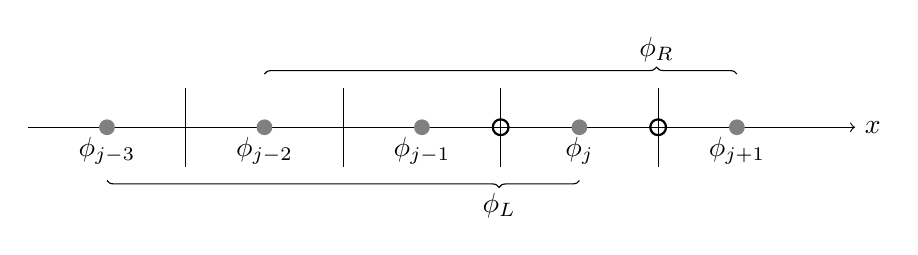
\begin{tikzpicture}[
  cpnt/.style={fill=gray},
]

\draw [->] (-5,0) -- (5.5,0) node [right] {$x$};
\draw (-3,-0.5) -- (-3,0.5);
\draw (-1,-0.5) -- (-1,0.5);
\draw (1,-0.5) -- (1,0.5);% node [above] {$\phi_L$};
\draw (3,-0.5) -- (3,0.5);% node [above] {$\phi_R$};

\draw[decoration={brace,mirror,raise=5pt,aspect=0.83}, decorate] (-4,-0.5) -- node[below=6pt,pos=0.83] {$\phi_L$} (2,-0.5);
\draw[decoration={brace,raise=5pt,aspect=0.83}, decorate] (-2,0.5) -- node[above=6pt,pos=0.83] {$\phi_R$} (4,0.5);

\path [cpnt] (-4,0) circle [radius=0.1] node [below] {$\phi_{j-3}$};
\path [cpnt] (-2,0) circle [radius=0.1] node [below] {$\phi_{j-2}$};
\path [cpnt] (0,0) circle [radius=0.1] node [below] {$\phi_{j-1}$};
\path [cpnt] (2,0) circle [radius=0.1] node [below] {$\phi_j$};
\path [cpnt] (4,0) circle [radius=0.1] node [below] {$\phi_{j+1}$};
\draw [thick] (1,0) circle [radius=0.1];
\draw [thick] (3,0) circle [radius=0.1];

\end{tikzpicture}
	\caption{The one-dimensional cubicFit transport scheme interpolates face values $\phi_L$ and $\phi_R$ using four-point, upwind-biased stencils of cell-centre values.}
	\label{fig:cubicFit}
\end{figure}

The one-dimensional cubic interpolation is
\begin{align}
	\phi = a_1 + a_2 x + a_3 x^2 + a_4 x^3 \text{.} \label{eqn:cubic}
\end{align}
Assuming a uniform mesh with $\Delta x = 1$ and choosing the position of $\phi_{i+1/2}$ to be $x=0$, equation~\eqref{eqn:cubic} is evaluated at the cell centres $\phi_{i-2}, \ldots, \phi_{i+1}$ to form the matrix equation
\begin{align}
	\mathbf{B} \mathbf{a} &= \bm{\phi} \\
	\begin{bmatrix}
		1 & -5/2 & 25/4 & -125/8 \\
		1 & -3/2 &  9/4 & -27/8 \\
		1 & -1/2 &  1/4 &  -1/8 \\
		1 &  1/2 &  1/4 &   1/8 \\
	\end{bmatrix}
	\begin{bmatrix}
		a_1 \\
		a_2 \\
		a_3 \\
		a_4
	\end{bmatrix}
	&=
	\begin{bmatrix}
		\phi_{i-2} \\
		\phi_{i-1} \\
		\phi_i \\
		\phi_{i+1}
	\end{bmatrix} \text{.}
\end{align}
The unknown coefficients $\mathbf{a}$ are found by inverting $\mathbf{B}$ such that $\mathbf{a} = \mathbf{B}^{-1} \bm{\phi}$.  The inverse matrix is
\begin{align}
	\mathbf{B}^{-1} = 
	\frac{1}{48}
	\begin{bmatrix}
		3 & -15 & 45 & 15 \\
		2 & -6 & -42 & 46 \\
		-12 & 60 & -84 & 36 \\
		-8 & 24 & -24 & 8
	\end{bmatrix} \label{eqn:cubicfit-inverse}
\end{align}
Since $x=0$ was chosen to be the position $i+1/2$ then 
\begin{align}
	\phi_{i+1/2} = a_1 = 
	\frac{1}{16}
	\begin{bmatrix}
		1 \\ -5 \\ 15 \\ 5
	\end{bmatrix}
	\cdot
	\begin{bmatrix}
		\phi_{i-2} \\
		\phi_{i-1} \\
		\phi_i \\
		\phi{i+1}
	\end{bmatrix} \text{.} \label{eqn:cubicfit-fluxcoeffs}
\end{align}

The finite difference method offers another way to discretise the flux divergence of cell $i$ with a cubic approximation using cell centre values $\phi_{i-2}, \ldots, \phi_{i+1}$.  A matrix equation is constructed using equation~\eqref{eqn:cubic} evaluated at every cell centre.  For convenience, assume that $\Delta x = 1$ and that $x=0$ at the cell centre position of $\phi_i$, hence the matrix equation becomes
\begin{align}
	\mathbf{B} \mathbf{a} &= \bm{\phi} \\
	\begin{bmatrix}
		1 & -2 & 4 & -8 \\
		1 & -1 & 1 & -1 \\
		1 &  0 & 0 &  0\\
		1 &  1 & 1 &  1\\
	\end{bmatrix}
	\begin{bmatrix}
		a_1 \\
		a_2 \\
		a_3 \\
		a_4
	\end{bmatrix}
	&=
	\begin{bmatrix}
		\phi_{i-2} \\
		\phi_{i-1} \\
		\phi_i \\
		\phi_{i+1}
	\end{bmatrix}
\end{align}
The unknown coefficients $\mathbf{a}$ are found by calculating the inverse matrix,
\begin{align}
	\mathbf{B}^{-1} = 
	\frac{1}{6}
	\begin{bmatrix}
		0 & 0 & 6 & 0 \\
		1 & -6 & 3 & 2 \\
		0 & 3 & -6 & 3 \\
		-1 & 3 & -3 & 1
	\end{bmatrix}
\end{align}
To calculate the flux divergence I calculate the derivative $\partial \phi / \partial x = a_2 + 2 a_3 x + 3 a_4 x^2$.  Evaluating the flux divergence at $\phi_i$ where $x=0$ then $\partial \phi_i / \partial x = a_2$.  Hence I find that the finite difference weighted sum is
\begin{align}
	-u \frac{\partial \phi_i}{\partial x} = -u a_2 =
	-u \cdot \frac{1}{6}
	\begin{bmatrix}
		1 \\ -6 \\ 3 \\ 2
	\end{bmatrix}
	\cdot
	\begin{bmatrix}
		\phi_{i-2} \\
		\phi_{i-1} \\
		\phi_i \\
		\phi_{i+1}
	\end{bmatrix} \label{eqn:fd-fluxdiv}
\end{align}
The cubic finite difference approximation given in equation~\eqref{eqn:fd-fluxdiv} is conservative on uniform meshes.  This can be demonstrated by decomposing the weights vector,
\begin{align}
	-u \cdot \frac{1}{6}
	\begin{bmatrix}
		1 \\ -6 \\ 3 \\ 2
	\end{bmatrix}
	\cdot
	\begin{bmatrix}
		\phi_{i-2} \\
		\phi_{i-1} \\
		\phi_i \\
		\phi_{i+1}
	\end{bmatrix}
	&= 
	-u \cdot
	\frac{1}{6}
	\left(
	\begin{bmatrix}
		0 \\ -1 \\ 5 \\ 2
	\end{bmatrix}
	-
	\begin{bmatrix}
		-1 \\ 5 \\ 2 \\ 0
	\end{bmatrix}
	\right)
	\cdot
	\begin{bmatrix}
		\phi_{i-2} \\
		\phi_{i-1} \\
		\phi_i \\
		\phi_{i+1}
	\end{bmatrix} \\
	&=
	-u \left(
	\frac{1}{6}
	\begin{bmatrix}
		-1 \\ 5 \\ 2
	\end{bmatrix}
	\cdot
	\begin{bmatrix}
		\phi_{i-1} \\
		\phi_i \\
		\phi_{i+1}
	\end{bmatrix}
	-
	\frac{1}{6}
	\begin{bmatrix}
		-1 \\ 5 \\ 2
	\end{bmatrix}
	\cdot
	\begin{bmatrix}
		\phi_{i-2} \\
		\phi_{i-1} \\
		\phi_i
	\end{bmatrix} \right) \text{.} \label{eqn:fd-fluxcoeffs}
\end{align}
Notice that the flux divergence has been rewritten as the difference between right and left fluxes (equation~\ref{eqn:fluxdiv}).

\subsection*{Calculating the high-order correction}
The high-order correction to the cubicFit scheme is calculated as the difference between the cubic finite difference approximation (equation~\ref{eqn:fd-fluxcoeffs}) and the uncorrected cubicFit approximation (equation~\ref{eqn:cubicfit-fluxcoeffs}),
\begin{align}
	\mathrm{correction}(\phi_{i+1/2})
	&=
	\left(
	\frac{1}{6} 
	\begin{bmatrix}
		0 \\ -1 \\ 5 \\ 2
	\end{bmatrix}
	-
	\frac{1}{16}
	\begin{bmatrix}
		1 \\ -5 \\ 15 \\ 5
	\end{bmatrix}
	\right)
	\cdot
	\begin{bmatrix}
		\phi_{i-2} \\
		\phi_{i-1} \\
		\phi_i \\
		\phi_{i+1}
	\end{bmatrix} \\
	&=
	\frac{1}{48}
	\begin{bmatrix}
		-3 \\ 7 \\ -5 \\ 1
	\end{bmatrix}
	\cdot
	\begin{bmatrix}
		\phi_{i-2} \\
		\phi_{i-1} \\
		\phi_i \\
		\phi_{i+1}
	\end{bmatrix} \label{eqn:correction} \\
%
\intertext{which can be decomposed into a linear combination of second derivatives where $\partial_x^2 \phi_i = \phi_{i-1} - 2 \phi_i + \phi_{i+1}$,}
%
	&=
	\frac{1}{48} \left(
	-3 \begin{bmatrix}1 \\ -2 \\ 1 \\ 0\end{bmatrix}
	+ \begin{bmatrix}0 \\ 1 \\ -2 \\ 1\end{bmatrix}
	\right)
	\cdot
	\begin{bmatrix}
		\phi_{i-2} \\
		\phi_{i-1} \\
		\phi_i \\
		\phi_{i+1}
	\end{bmatrix} \\
	&=
	\frac{1}{48}
	\left( -3 \partial_x^2 \phi_{i-1} + \partial_x^2 \phi_i \right)
\end{align}
Applying this correction using the three-point approximation of the second derivative results in third-order convergence on uniform meshes and second-order convergence on non-uniform meshes.

Alternatively, the second derivative can be calculated from equation~\eqref{eqn:cubic} such that $\partial_x^2 \phi = 2a_3 + 6a_4x$ where $a_3$ and $a_4$ can be calculated using equation~\eqref{eqn:cubicfit-inverse}.  This approach results in fourth-order convergence on uniform meshes and second-order convergence on non-uniform meshes.  Curiously, this approach yields the correction
\begin{align}
	\mathrm{correction}(\phi_{i+1/2})
	&=
	\frac{1}{48}
	\begin{bmatrix}
		0.975 \\ -4.925 \\ 6.925 \\ -2.975
	\end{bmatrix}
	\cdot
	\begin{bmatrix}
		\phi_{i-2} \\
		\phi_{i-1} \\
		\phi_i \\
		\phi_{i+1}
	\end{bmatrix} 
	\approx
	\frac{1}{48}
	\begin{bmatrix}
		1 \\ -5 \\ 7 \\ -3
	\end{bmatrix}
	\cdot
	\begin{bmatrix}
		\phi_{i-2} \\
		\phi_{i-1} \\
		\phi_i \\
		\phi_{i+1}
	\end{bmatrix}
\end{align}
whose coefficients are similar to those in equation~\ref{eqn:correction}.


\bibliographystyle{ametsoc2014}
\bibliography{references}

\end{document}
